
\documentclass{beamer}
\usepackage{HECbeamer}
% \usepackage{pgfpages}
% \pgfpagesuselayout{4 on 1}[letterpaper, landscape, border shrink=5mm]
\title[\color{white}{MATH 60604A \S~4f - Overdispersed count data}]{\texorpdfstring{MATH 60604A \\Statistical modelling \\ \S~4f - Overdispersed count data}{MATH 60604A \\Statistical modelling \\ \S~4f - Overdispersed count data}}
\author{Léo Belzile}
\institute{HEC Montréal\\
Department of Decision Sciences}
\date{} 

\begin{document}
\frame{\titlepage}

\begin{frame}[fragile]
\frametitle{Extensions to Poisson to deal with overdispersion}
\bi
\item The Poisson distribution is not very flexible, because it only includes one parameter, which is equal to both the mean and the variance.
\item In most cases, this assumption is not valid. In the previous output, the deviance divided by the degrees of freedom was $203.2710/110 = 1.85$, suggesting  the Poisson model is \textbf{not adequate} ($p$-value less than $10^{-5}$).
\item The underlying reason is that the observed variability in counts is much larger than the mean in this example, a phenomenon termed \textbf{overdispersion}.
\item The \alert{negative binomial} model if often used as replacement for overdispersed count data.
\ei
\end{frame}


\begin{frame}[fragile]
\frametitle{Negative binomial distribution}
\bi
\item The negative binomial distribution is a probability distribution for \alert{integer} random variables with two parameters.
\item We restrict attention the most common parametrization used in modelling. The probability mass function is
\begin{align*}
\P{Y=y}=\frac{\Gamma(y+1/k)}{\Gamma(y+1)\Gamma(1/k)} \left(\frac{1/k}{1/k + \mu} \right)^{1/k} \left(\frac{\mu}{1/k+\mu}\right)^y
\end{align*}
for $y=0, 1, 2, 3, \ldots$, where $\Gamma$ denotes the gamma function. Both parameters are positive, meaning $\mu>0$ and $k>0$.

\item The mean and the variance are \begin{align*}
\E{Y}=\mu, \qquad \Va{Y}=\mu+k\mu^2.                                 \end{align*}
\item The variance of the negative binomial distribution is always \alert{larger} than its mean. 
\ei
\end{frame}


\begin{frame}[fragile]
\frametitle{Negative binomial regression}
\bi
\item Negative binomial regression usually assumes that the response variable $Y$ 
follows a \alert{negative binomial} distribution and that the \alert{link function} is the logarithmic function 
\begin{align*}
g\{\E{Y_i}\}=\log\{\E{Y_i}\}=\beta_0+\beta_1\mathrm{X}_{i1}+\ldots+\beta_p\mathrm{X}_{ip}.
\end{align*}
\item Equivalently, we assume that each observation $Y_i$ follows a negative binomial distribution with mean
\begin{align*}
\E{Y_i}=\exp(\beta_0+\beta_1\mathrm{X}_{i1}+\ldots+\beta_p\mathrm{X}_{ip})
\end{align*}
\item The interpretation of the parameters is the same as for Poisson regression. 

\item There is a second parameter, $k$, which is assumed to be \alert{the same for every observation} and therefore doesn't depend on the predictor variables.
\ei

{ \tiny Mathematical aside:
The negative binomial model is not a generalized linear model per say because it is part of exponential-dispersion family, but we can use maximum likelihood and the GLM machinery to fit the model.

}
\end{frame}



\begin{frame}[fragile]
\frametitle{Negative binomial regression with \code{proc genmod}}
The only difference from the Poisson model is that we specify \texttt{dist=negbin}.
\begin{tcolorbox}[colback=white, colframe=hecblue, title=SAS code to fit a negative binomial model]
% proc glimmix data=statmod.regdenombrement1;
% class educ revenu;
% model nombreachat=sexe age revenu educ statut 
%      fixation emotion / dist=negbin link=log solution;
% run;
\begin{verbatim}
proc genmod data=statmod.intention;
class educ revenue;
model nitem=sex age revenue educ marital
     fixation emotion / dist=negbin link=log lrci;
run;
\end{verbatim}
\end{tcolorbox}
{\footnotesize
In \Rlang, the parametrization of \texttt{MASS::glm.nb} is such that $\theta=1/k$.


}
\end{frame}

\begin{frame}[fragile]
\frametitle{Goodness-of-fit diagnostics for negative binomial}
\begin{center}
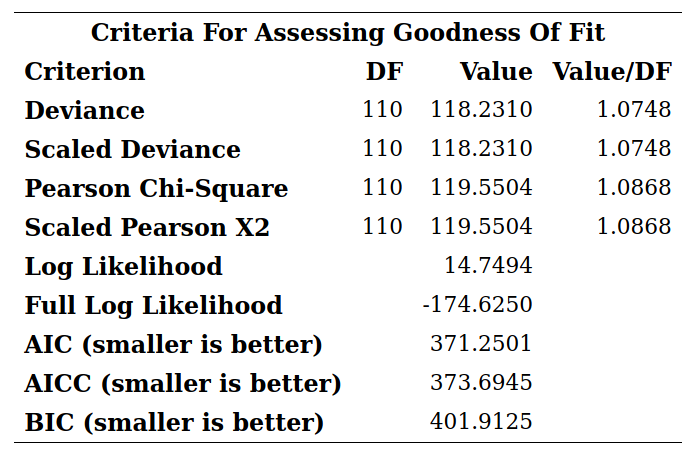
\includegraphics[width = 0.55\linewidth]{img/c4/slides8-e6}
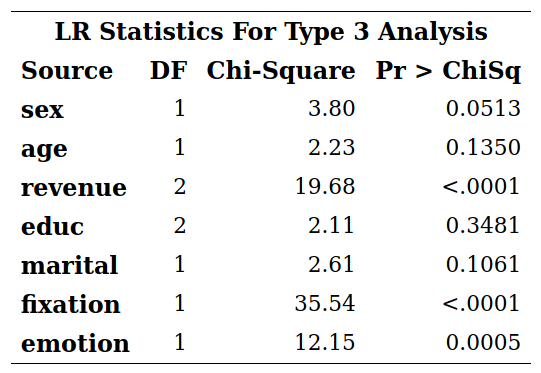
\includegraphics[width = 0.44\linewidth]{img/c4/slides8-e7}
\end{center}
The deviance over degrees of freedom is closer to unity. Only \texttt{revenue}, \texttt{fixation} and \texttt{emotion} are statistically significant.
\end{frame}

\begin{frame}[fragile]
\frametitle{Parameter estimates for the negative binomial model}
\begin{center}
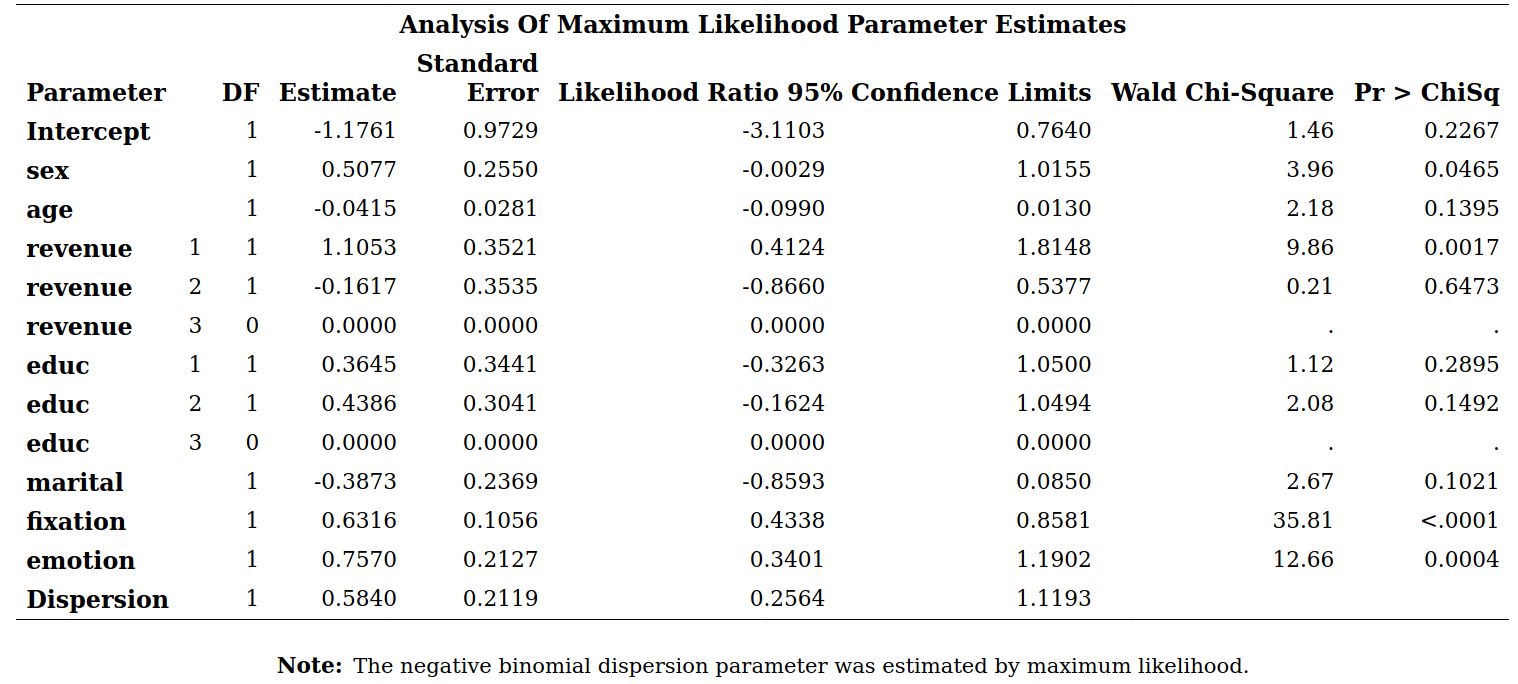
\includegraphics[width = 0.99\linewidth]{img/c4/slides8-e8}
\end{center}
{\footnotesize 
The scale parameter $\hat{k} = 0.584$. Note that the likelihood-ratio based 95\% confidence interval may lead to different inference than the Wald tests and their $p$-values; prefer the former as they are more reliable.


}
\end{frame}

\begin{frame}[fragile]
\frametitle{Model selection}
\bi
\item The deviance indicates that the negative binomial model is preferable to the Poisson, but this is informal.
\item Another to answer this would be to look at information criteria (smaller is better): the negative binomial model is selected by both $\mathsf{AIC}$ and $\mathsf{BIC}$.
\ei
\begin{center}
\begin{tabular}{crr}
\toprule
 Model & \multicolumn{1}{c}{Poisson} & \multicolumn{1}{c}{neg. binom.}
 \\ \midrule
 $\mathsf{AIC}$ & $392.33$ & $371.25$ \\
$\mathsf{BIC}$ & $420.20$ & $301.91$ \\\bottomrule
\end{tabular}
\end{center}


\end{frame}

\begin{frame}[fragile]
\frametitle{Negative binomial distribution versus Poisson}
\bi

\item As $k$ approaches zero, we recover the
Poisson distribution. 
\item We can actually compare these two models using the likelihood ratio test since they are nested. 
\item  We can test the hypotheses $\Hy_0: k=0, \Hy_1: k\neq 0$ using a likelihood ratio test
\bi \item beware! the null distribution is \textbf{non-regular} because when $n \to \infty$, there is a $0.5$ probability that the deviance will be exactly zero and $0.5$ that it follows a $\chi^2_1$ under $\Hy_0$.
\ei
\item The asymptotic null distribution is 
\begin{align*}
2\{\ell_{\mathsf{negbin}}(\hat{\mu}_{\mathsf{negbin}}, \hat{k}) - \ell_{\mathsf{pois}}(\hat{\mu}_{\mathsf{pois}})\} \stackrel{\cdot}{\sim} \frac{1}{2}\chi^2_1 + \frac{1}{2} \delta_0;
\end{align*}
Practical aspect: if we do not observe $\hat{k}=0$, we calculate the $p$-value as usual using the $\chi^2_1$ distribution and \textbf{divide it by two} to get the \textbf{correct result}.
\ei
\end{frame}
\begin{frame}[fragile]
\frametitle{Likelihood ratio test (non-regular)}
This shows how to to the calculations by hand using the output from the tables.
\bi \item The ``\textbf{Full Log Likelihood}'' give the fitted likelihood of the model, $-174.6250$ for the negative binomial model and $-186.1639$ for the Poisson model.
\item The difference is $11.5389$ and the likelihood ratio statistic is $23.08$.
\item The probability that a  $\chi^2_1$ is larger than $23.08$ is $1.55 \times 10^{-7}$.
\item Since the problem is non-regular, we halve this probability and so our $p$-value is $7.7 \times 10^{-8}$. 
\ei
\begin{tcolorbox}[colback=white, colframe=hecblue, title=SAS code for likelihood ratio test (non-regular)]
{\small 
\begin{verbatim}
data pval;
pval=(1-CDF('CHISQ',23.08,1))/2;
run;
proc print data=pval;
run;
\end{verbatim}
}
\end{tcolorbox}
{\footnotesize There is overwhelming evidence that the negative binomial model is preferable.

}

\end{frame}


\end{document}
